\documentclass{beamer}
\usepackage[brazil]{babel}
%\usepackage[latin1]{inputenc}
\usepackage[utf8x]{inputenc} 
%\usepackage[all]{xy}
\PrerenderUnicode{ç}

\setbeamercovered{transparent=5}

\usetheme{Antibes}

\title{Projeto de Tradução do GNOME para o Português do Brasil: presente e futuro}

\author{Rodrigo L. M. Flores \\ \url{mail@rodrigoflores.org}}

\logo{
\includegraphics[width=1cm]{figures/gnome-logo}}

\institute{GNOME Brasil}
\begin{document}

\date{\today}

\frame{\titlepage}

\frame{\tableofcontents}

\begin{frame}
    \frametitle{Nosso status}    
    \begin{itemize}[<+->]
        \item \color[rgb]{0,1,0} Somos citados nas notas de lançamento desde o GNOME 2.4 (Setembro de 2003)  
        \item \color[rgb]{0,1,0} 100\% da Interface do Oficial 
        \item \color[rgb]{0,1,0} 87\% da Interface do Extra
        \item \color[rgb]{0,1,0} 82\% da Interface de Infraestrutura
        \item \color[rgb]{1,0,0} 36\% de Documentação do Oficial
        \item \color[rgb]{1,0,0} 9\%  de Documentação do Extra
        \item \color[rgb]{1,0,0} 31\% de Documentação de Infraestrutura
    \end{itemize}
\end{frame}

\section{Passado}

\begin{frame}
    \frametitle{E onde está o passado ?}
    Informações incertas demais para se falar ! Entrei em dezembro de 2007, então muita gente eu não tive
    o prazer de trabalhar junto. 
\end{frame}

\begin{frame}
    \frametitle{Mas sem esquecer de citar}
    \begin{columns}[c]
      \column{1.5in}
        \begin{itemize}
          \item Alexandre Folle de Menezes
          \item André Noel
          \item Estevão Procópio
          \item Evandro Giovanini
          \item Guilherme Pastore
          \item Gustavo Noronha
          \item Hugo Dória
       \end{itemize}
       \column{1.5in}
       \begin{itemize}
          \item Igor Soares
          \item Maurício Collares
          \item Luiz Armesto
          \item Pedro de Medeiros
          \item Raphael Higino
          \item Raul Pereira
          \item Sandro Nunes Henrique 
          \item Washington Lins
        \end{itemize}
    \end{columns}
\end{frame}

\section{Um pouco sobre nós}

\begin{frame}
    \frametitle{Missão}
    Fazer com que usuários do GNOME possam utilizar um sistema 
    totalmente traduzido para nosso idioma, cumprindo 
    com padrões altos de qualidade 
\end{frame}

\begin{frame}
  \frametitle{E o que o GNOME ganha com isso ?}
  \begin{itemize}
    \item Mais usuários
    \item Maior ``acessibilidade''
  \end{itemize}  
\end{frame}

\begin{frame}
  \frametitle{E o que nós ganhamos com isso?}
  \begin{itemize}
    \item Orgulho de termos nosso nome nos créditos do GNOME;
    \item Oportunidade para aprender a traduzir um software;
    \item Aprendemos sobre as ferramentas do GNOME;
    \item Derrubamos ainda mais o mito que precisa ser um hacker pra usar Linux;
  \end{itemize}
\end{frame}


\section{Como funcionávamos ?}

\begin{frame}
    \frametitle{Nosso fluxo de trabalho antigo}
    \begin{figure}[ht]
        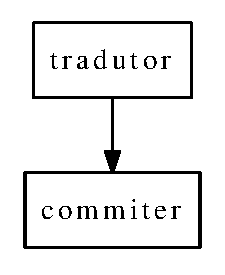
\includegraphics{figures/fluxo_antigo.eps}     
    \end{figure}
\end{frame}

\begin{frame}
    \frametitle{Fluxo de tradução antigo}
    \begin{enumerate}[<+->]
        \item Tradutor escolhe um módulo não reservado no Wiki
        \item Tradutor baixa o arquivo po no Damned Lies
        \item Tradutor traduz o arquivo po
        \item Tradutor envia o arquivo po ao Bugzilla
        \item Commiter revisa a tradução 
        \item Commiter envia ao Bugzilla e marca o ``bug'' como resolvido
        \item Commiter faz o commit no SVN
    \end{enumerate}
\end{frame}

\begin{frame}
    \frametitle{Falhas?}
    \begin{itemize}[<+->]
        \item Processo muito dependente do commiter
        \item Reservas no Wiki as vezes eram esquecidas e aí módulos estavam ``pseudo-reservados''
        \item Processo muito complicado
    \end{itemize}
\end{frame}

\section{Uma nova era...}

\begin{frame}
    \frametitle{O que tinhamos?}
    \begin{itemize}[<+->]
        \item Tradutores experientes;
        \item Vertimus;
    \end{itemize}
\end{frame}

\begin{frame}
    \frametitle{Nova proposta}  
    Em Abril de 2008, o Leonardo Fontenelle sugeriu uma nova proposta de organização da equipe:
    \begin{itemize}[<+->]
        \item Criação de uma nova classe: o revisor
        \item Promoção de um tradutor para revisor dependentemente principalmente dos outros revisores/committers
        \item Confiança no revisor
    \end{itemize}
\end{frame}


\begin{frame}
    \frametitle{E como tradutores viram revisores?}
    Através de um pedido na lista.

    Requisitos:
    \begin{itemize}[<+->]
        \item Fazer parte da equipe há, pelo menos, 6 meses
        \item Ser aprovado por pelo menos 2 revisores (e o coordenador pode ser um desses)
        \item Ser aprovado pelo coordenador
    \end{itemize}
\end{frame}

\begin{frame}
    \frametitle{Novo fluxo de trabalho}
    \begin{figure}[ht]
        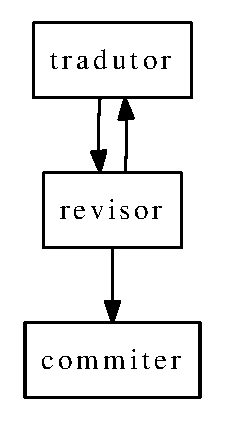
\includegraphics{figures/fluxo_novo.eps}     
    \end{figure}
\end{frame}

\begin{frame}
    \frametitle[Vertimus]{Novo fluxo de tradução}
    \begin{enumerate}[<+->]
        \item Tradutor reserva e baixa a tradução no Vertimus
        \item Tradutor sobe o arquivo traduzido ao Vertimus
        \item Revisor reserva a tradução
        \item Revisor sobe o arquivo revisado ao Vertimus
        \item Commiter baixa o arquivo do Vertimus
        \item Commiter avisa da submissão
    \end{enumerate}
\end{frame}

\begin{frame}
    \frametitle{Resolve os falhas antigas ?}
    \begin{itemize}[<+->]
        \item Ainda somos dependentes dos Commiters, mas só para enviar tradução.
        \item Ver traduções pendentes é mais simples
        \item Reserva do módulo é redefinida a cada commit
        \item Processo bem mais simples
    \end{itemize}
\end{frame}

\begin{frame}
    \frametitle{Processo ainda não é perfeito }
    \begin{itemize}[<+->]
        \item Dependente dos commiters (que tem que sempre rodar alguns comandos);
        \item Processo de baixar/traduzir/subir é meio chato;
        \item Burocracia de arquivos po;
        \item Trabalho não é versionado automaticamente;
        \item Faltam métricas
        \item Processo pode ficar ainda mais simples;
    \end{itemize}
\end{frame}

\section{Problemas técnicos}

\begin{frame}
  \frametitle{Falhas humanas acontecem...}
  \begin{figure}
    \includegraphics<1-2>[scale=0.5]{figures/Welsh.png}
    \includegraphics<3>[scale=0.5]{figures/translateservererror.jpg}
    \includegraphics<4>[scale=0.5]{figures/bugtraditunes8.png}
  \end{figure} 
  
  \only<2>{I am not in the office at the moment. Please send any work to be translated.}
  \only<2>{Retirado de \url{http://news.bbc.co.uk/2/hi/uk_news/wales/7702913.stm}}  
  \only<3>{Retirado de \url{http://kibeloco.com.br/kibeloco/2008/09/09/pracas-do-braziu-ou-melhor-da-xina/} }  
  \only<4>{Retirado de \url{http://appleaddicted.com.br/blog/erro-de-traducao-no-itunes-8/}}
\end{frame}

\begin{frame}
  \frametitle{As vezes de uma maneira mais sutil}
  \begin{itemize}[<+->]
    \item Padrões
    \item Typos
    \item Ortografia  
    \item Teclas de acesso rápido
    \item Termos ``importados''
    \item Erros frequentes
  \end{itemize}
\end{frame}

\begin{frame}
  \frametitle{Como evitar ?}

  \begin{itemize}[<+->]
    \item Traduzir com mais atenção
    \item Tradutor também deve revisar sua tradução
    \item Revisão mais detalhada do revisor
  \end{itemize}
\end{frame}

\begin{frame}
  \frametitle{Mas se algum erro passar...}
  Nos avise! Na próxima versão o erro certamente estará corrigido
  \begin{itemize}[<+->]
    \item E-mail
    \item Bugzilla
    \item IRC
  \end{itemize}
\end{frame}


\section{Dando nome aos bois}

\begin{frame}
    \frametitle{``Committers''}
    \begin{columns}
      \column{1.5in}
        \begin{itemize}
          \item<1-> John Wendell
          \item<2-> Leonardo Fontenelle 
          \item<3-> Og Maciel
        \end{itemize}
      \column{1.5in}
        \begin{figure}
          \includegraphics<1>[scale=0.5]{figures/jwendell.png}     
          \includegraphics<2>[scale=0.5]{figures/leonardof.png}     
          \includegraphics<3>[scale=0.5]{figures/ogmaciel.png}     
        \end{figure}
    \end{columns}
\end{frame}

\begin{frame}[fragile]
    \frametitle{Revisores}
    \begin{columns}
      \column{1.5in}
        \begin{itemize}
          \item<1-> Todos os committers
          \item<2-> Djavan Fagundes
          \item<3-> Fábio Nogueira
          \item<4-> Fabrício Godoy
          \item<5-> Henrique Machado    
          \item<6-> Vladimir Melo 
        \end{itemize}
      \column{1.5in}
        \begin{figure}
          \includegraphics<3>[scale=0.5]{figures/fnogueira.png} 
          \includegraphics<5>[scale=0.5]{figures/zehrique.png} 
          \includegraphics<6>[scale=0.5]{figures/vmelo.png}     
        \end{figure}

    \end{columns}
\end{frame}

\begin{frame}[fragile]
    \frametitle{Tradutores}
    \begin{columns}[c]
      \column{1.5in}

      \begin{itemize}
        \item Todos os revisores;
        \item<1-> André Gondim
        \item<2-> Carlos Pereira
        \item<3-> César Veiga
        \item<4-> Daniel Koda
        \item<5-> Enrico Nicoletto
        \item<6-> Flamarion Jorge
        \item<7-> Isis Binder
        \item<8-> Jader Henrique 
      \end{itemize}
      \column{1.5in}
        \begin{figure}
          \includegraphics<1>{figures/gondim.png}     
        \end{figure}

    \end{columns}
\end{frame}


\begin{frame}[fragile]
    \frametitle{Tradutores}
    \begin{columns}[c]
      \column{1.5in}
      \begin{itemize}
        \item<1-> Krix Apolinário
        \item<2-> Luciano Gardim
        \item<3-> Lucas Azevedo
        \item<4-> Michel Recondo
        \item<5-> Rodolfo Gomes
        \item<6-> Taylon Silmer
        \item<7-> Tiago Casal
        \item<8-> Wancharle Quirino 
      \end{itemize}
      \column{1.5in}
        \begin{figure}
          \includegraphics<3>{figures/lucasazevedo.png}     
        \end{figure}


    \end{columns}
\end{frame}

\section{LDP-BR}

\begin{frame}
  \frametitle{O que é?}
  \begin{itemize}[<+->]
    \item Linux Documentation Project - Brasil
    \item Lista de discussão
    \item Vocabulário Padrão (VP)
    \item Projeto de tradução de documentações e aplicativos
  \end{itemize}
\end{frame}

\section{Futuros planos}

\begin{frame}
    \frametitle{Iniciantes?}
    Nossa equipe tem um forte incentivo à entrada de iniciantes. Para isso poderia haver um ``plano de iniciação''.
    \begin{enumerate}
        \item Corrigir e traduzir pequenas coisas, normalmente adições de strings ou corrigir erros. 
        \item Traduzir interface mais simples (faltando menos de 20 strings)
        \item Traduzir interface mais complexos 
        \item Traduzir interfaces do zero
        \item Traduzir documentações conhecidas
    \end{enumerate}
\end{frame}

\begin{frame}
    \frametitle{Reforma ortográfica}

    Nosso plano: O GNOME 3.0 ser lançado nas novas normas de ortografia. 

\end{frame}

\begin{frame}
    \frametitle{Tradução incremental de documentações grandes}
    Algumas documentações têm centenas de mensagens, boa parte delas do tamanho de parágrafos. 
    Será que um envio incremental não ajudaria a melhorar a qualidade delas?
\end{frame}

\begin{frame}
    \frametitle{Revisão obrigatória para traduções grandes}
    Quanto maior a tradução, maior a chance de pequenos erros persistirem. 
    Não seria bom as traduções grandes serem revisadas independentementes do tradutor?
\end{frame}

\begin{frame}
    \frametitle{Melhorar nosso wiki}
    É de lá que as pessoas conhecem nosso trabalho! Temos que melhorar bastante :-).
\end{frame}

\begin{frame}
  \frametitle{Projetos relacionados}
  \begin{itemize}
    \item GNOME Translation Project
    \item LDP-BR
  \end{itemize}
\end{frame}

\begin{frame}
  \frametitle{Melhoras para o VP}
  Um sistema web
  \begin{itemize}[<+->]
    \item Votação online de termos
    \item Propôr traduções padrão
    \item Feedback de traduções atuais 
  \end{itemize}
\end{frame}

\section{Finais...}

\begin{frame}
  \frametitle{Junte-se a nós}
  Nós estamos sempre abertos a novos tradutores!
  \begin{block}{Links}
     \url{http://br.gnome.org/GNOMEBR/Traducao}\\
     \url{http://l10n.gnome.org}
  \end{block}
\end{frame}


\begin{frame}
  \frametitle{Agradecimentos}

  \begin{itemize}[<+->]
    \item Todos os tradutores e revisores da equipe;
    \item Izabel Valverde;
    \item Fundação GNOME;     
  \end{itemize}
\end{frame}

\begin{frame}
    \begin{block}{Contato}     
    \begin{itemize}
            \centering
            \item[E-mail] mail@rodrigoflores.org 
            \item[XMPP]  im@rodrigoflores.org        
            \item[Site]  \url{http://rodrigoflores.org}
            \item[Blog]  \url{http://blog.rodrigoflores.org}        
            \item[Twitter] rlmflores 
            \item[Identi.ca] rodrigoflores        
            \item[Jaiku] flores        
        \end{itemize}
    \end{block}
\end{frame}


\end{document}


% vim:set ts=2 expandtab:
